\begin{center}
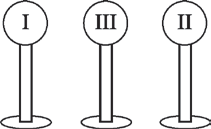
\includegraphics[scale=0.5]{images/img-004-014.png}
\end{center}

% Multiple Choice Question 14
\begin{questions}\setcounter{question}{13}\question
Three identical conducting spheres are mounted on insulating handles, as shown above. Spheres I and II have equal charges of $+Q$ and are separated by a fixed distance. They repel each other with an electrostatic force of magnitude $F$. Sphere III, initially uncharged, is first touched to sphere I, then to sphere II, and then removed. If the charge distribution on each sphere is assumed to always be spherical, the new magnitude of the electrostatic force between spheres I and II is

\begin{oneparchoices}
\choice Zero
\choice $\dfrac{F}{16}$
\choice $\dfrac{F}{4}$
\choice $\dfrac{F}{2}$
\choice $\dfrac{3 F}{8}$
\end{oneparchoices}\end{questions}

